\section{From Parametrized Surface Points to NURBS Representation}
\todourgent[author=Benni,inline]{@ Benni, Erik: refactor wrt wording}
As of yet, there is no open-source software which provides the conversion from a \textit{mesh-based} geometry to NURBS representation. Hence, one of the main challenges of both the algorithmic and implementation part of this project has been to develop one from scratch. Due to a variety of possible approaches to tackle this problem (e.g. \cite{eck1996automatic, becker2011advanced}), we conducted extensive prototyping work in MATLAB \cite{MATLAB} to avoid cumbersome and time-consuming implementation overheads during the prototyping phase. Once the algorithms were finalized, the prototypes were implemented in a non-proprietary language, Python. 

In the following section, we will thus present the final algorithm, based on the theory in \autoref{sec:NURBS} and \autoref{sec:LSQfitting}\footnote{For reference, the nomenclature used in these sections is also used here.}. For a short overview, we settled on using Peters' scheme (\autoref{subsec:peters}) to fit NURBS smoothly to datapoints (\autoref{subsub:petersleastsq}) with an included fairness term (\autoref{subsec:fairnessthry} and \autoref{subsec:lsqfairness}). A similar approach was tried by Eck and Hoppe in \cite{eck1996automatic}, for unstructured point clouds.

\subsection{Algorithm}
For the input:
\begin{itemize}
\item a quadrilateral mesh of vertices ($\petersControlMeshVec \in \petersControlMesh$),
\item how they are connected into quads ($\verticesof{\hat{f}}, \forall \hat{f} \in \petersFaces$) as an ordered list of four vertex indices,
\item a set of a datapoints ($\lsDataPoint_k \in \mathbb{R}^d$),
\item how they are parameterized (parameters $(u_{\lsDataPoint_k}, v_{\lsDataPoint_k})$ and on which quad $\hat{f}\in\petersFaces$),
\end{itemize}
the algorithm proceeds as follows (see \autoref{fig:petersAlgorithm} for a graphical overview):
\begin{figure}
\begin{center}
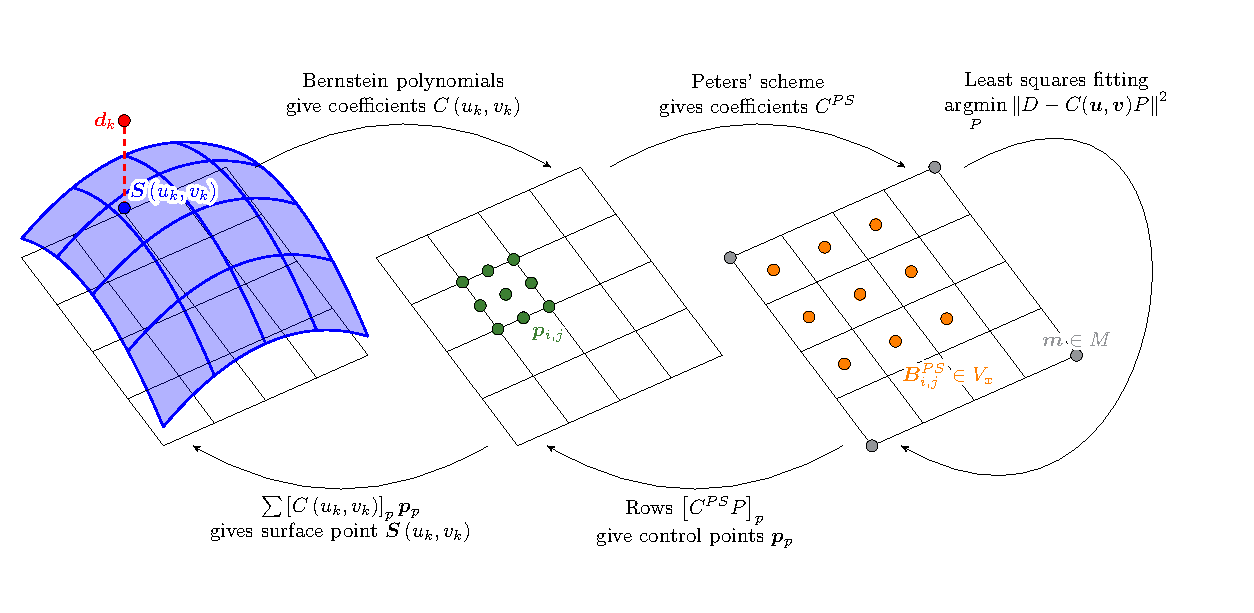
\includegraphics[width=1.1\textwidth]{Pictures/tikzPeters/Peterscombined.pdf}
\end{center}
\caption{Visualisation of the basic surface fitting algorithm, shown for one datapoint $\lsDataPoint_k$. The algorithm takes the parameterized input points $\lsDataPoint_k \in \mathbb{R}^d$, and produces a network of \Bez patches with control points $\vec{p}_{i,j}$, that can be used to create a surface. The steps can be followed in detail in the text. In the actual algorithm, a subsequent step combines the $4\times4$ \Bez surface patches on a quad (shown) into one NURBS patch.}
\label{fig:petersAlgorithm}
\end{figure}
%The algorithm is given information about a quadrilateral mesh of vertices ($\petersControlMeshVec \in \petersControlMesh$), how they are connected into quads ($\verticesof{\hat{f}}, \forall \hat{f} \in \petersFaces$) as an ordered list of four vertex indices, and how they are parameterized (parameters $(u_\lsDataPoint, v_\lsDataPoint)$ and on which quad $\hat{f}\in\petersFaces$). The algorithm then roughly proceeds as follows:
\begin{enumerate}
\item For every quad in the mesh, a $4 \times 4$ grid of points ($\petersPatchPoints$) is created. In addition, several lists are created for labelling these points. These labels define the position of the points with respect to each other and to corners on the quads. They are used later in the algorithm, where information about neighbouring points is needed\footnote{These labels are correlating with points $A, B \text{ and } C$ in \cite{peters1992constructing} and \cite{eck1996automatic}, for reference.}.
\item The matrix $\lsControlPointCoefMatrix(\vec{u},\vec{v})\lsControlPointCoefMatrix^{PS}$ containing coefficients between the datapoints $\lsDataPoint_k$ and the fitted points in $\petersPatchPoints$ is created.
\begin{enumerate}[label=(\alph*)]
\item For every datapoint $\lsDataPoint_k$ in the input, its parameters are first scaled from $\left[0,1\right]$ on the quad to $\left[0,1\right]$ on a local tensor product \Bez surface patch, related to the closest point in $\petersPatchPoints$. Then, the coefficients on the \Bez control points of this patch (corresponding to the datapoint's row in $\lsControlPointCoefMatrix(\vec{u},\vec{v})$) are calculated using the Bernstein polynomials, as described in \autoref{sec:NURBS}. 
\item Then, the corresponding row in $\lsControlPointCoefMatrix(\vec{u},\vec{v})\lsControlPointCoefMatrix^{PS}$ is calculated, using a matrix-free formulation of $\lsControlPointCoefMatrix^{PS}$. This matrix-free formulation uses a combination of a precalculated table of coefficients for the points in Peter's scheme (calculated according to \cite{eck1996automatic}), together with the lookup of neighbouring points in $\petersPatchPoints$ saved in the beginning of the algorithm. 
\item The row of $\lsControlPointCoefMatrix(\vec{u},\vec{v})\lsControlPointCoefMatrix^{PS}$ is saved in a sparse matrix\footnote{The sparse matrices for the surface reconstructed part are implemented using SciPy \cite{SciPy}.}. 
\end{enumerate}
\item For every point in $\petersPatchPoints$ (that is, for every \Bez patch), the precalculated coefficients of the Fairness functional (calculation described in \autoref{subsec:lsqfairness}) are applied to the \Bez control points of the patch to create one row of $\lsControlPointCoefMatrix^{fair}$. Using the same matrix-free formulation as before, the corresponding row of $\lsControlPointCoefMatrix^{fair}\lsControlPointCoefMatrix^{PS}$ is calculated, and saved in another sparse matrix.
\item The fitting to datapoints and fairness functional parts are combined by concatenating the datapoint matrix $\lsDataPointMatrix$ with a 3-dimensional $0$--vector, to form $\lsDataPointConcMatrix$, and by concatenating $\lsControlPointCoefMatrix(\vec{u},\vec{v})\lsControlPointCoefMatrix^{PS}$ and  $\lsControlPointCoefMatrix^{fair}\lsControlPointCoefMatrix^{PS}$ vertically to form $\lsControlCoefConcMatrix(\vec{u},\vec{v})\petersControlPointCoefMatrix$.
\item The actual locations of the points in the mesh $\petersPatchPoints$ is calculated using sparse linear least squares\footnote{Also using SciPy.}.
\item The \Bez points of the patches are reconstructed from the points in $\petersPatchPoints$, quad-wise, using a matrix-free formulation of the second part of Peters' scheme, again together with the lookup of neighbouring points saved in the beginning of the algorithm.
\end{enumerate}
At this point, we already have the components necessary for a reconstructed surface, now formulated as a network of \Bez patches\footnote{Or \emph{tensor produduct \Bez surface patches}, of second and third order (quadratic and cubic). See \autoref{subsub:bezcurvsurf} for definition (\autoref{eq:bezsurface}).}. A sample result at this stage, showing the fitting of a surface to a toroidal shape defined implicitly for the \acs{DC} algorithm, is shown in \autoref{fig:fittingStructures}. 

However, for conveniece and usability, we convert them into one cubic tensor product NURBS curve surface patch per quad. That means the $4\times4$ \Bez patches per quad are turned into one cubic NURBS patch. 

\begin{enumerate}[resume]
\item The network of \Bez patches are combined to a network of NURBS patches.
\begin{enumerate} [label=(\alph*)]
\item First, for each quad, the quadratic \Bez patches on this quad are degree-raised\footnote{See for example \cite{bezDegRaise} for how to compute the control points of an equivalent \Bez curve with a higher degree.} to cubic in both directions.\tododone[author=erik]{add formula or reference to for example web page with a degree raising formula}
%
\item Then, we can combine the $4\times4$ \Bez patches of the quad into one cubic NURBS patch. This is done by inserting the \Bez control points in a $13\times13$ array, where the shared control points along the \Bez patch edges are only inserted in once (instead of once for each \Bez patch), and using the knot vector 
$(0, 0, 0, 0,$ $0.25, 0.25, 0.25,$ $0.5, 0.5, 0.5,$ $0.75, 0.75, 0.75,$ $1, 1, 1, 1)$, in both directions.%
%
\footnote{That the surfaces are the same can be verified using for example the formulae in pp. 115-116 of \cite{shikin1995handbook}. A conceptual explanation would be as follows: we formulate the \Bez surfaces as NURBS surfaces, and then connect them along the edges by changing the knot multiplicities. This can be done since the Bernstein polynomials can be recovered from the NURBS basis functions (by clamping at both ends, thus using knots $0$ and $1$ with multiplicities $N+1$ for an order $N$ curve having $N+1$ control points). Then, just as two clamped NURBS curves sharing one end point are combined easily into one curve (by concatenating the lists of control points, but putting the shared control point in only once, and concatenating the knot vectors, but reducing the multiplicity of the knot at the intersection to the order of the curve), we combine the curves along the surface in both directions to have a combined surface.}
%
%Since the control points along the shared edges are the same\footnote{}, this can be done by putting them in once, simply done by putting them once, giving the knots of triple multiplicitycurves through the \Bez patch edges will have knots of triple multiplicity, with quadruple multiplicity along the edges of a quad to clamp the curve. 
\tododone[inline]{Add any NURBS reference}
\end{enumerate}
\item The NURBS patches are returned as a list of control points and an ordered array of indices for what control points belong to which quad.
\end{enumerate}
%\item Implementations of the algorithm to calculate these \Bez point coefficients, as well as plotting them for debugging and visualisation
%\item \Bez curve and surface evaluation via calculating the coefficients on each \Bez control point from a set of parameters
%\item Algorithms to extract the necessary datapoints and parameters from the result data of the \acf{DC} algorithm in \autoref{ssec:DC}, using geometric conversions where necessary, and ignoring unusual datapoints
%\item An algorithm for using the four above algorithms to assemble the total coefficient matrix in \autoref{eqn:petersminimisation} in \autoref{subsub:petersleastsq}
%\item An application of MATLAB's built-in least squares minimisation tool to fit the resulting network of \Bez patches to the extracted surface.
%\end{itemize}

\begin{figure}
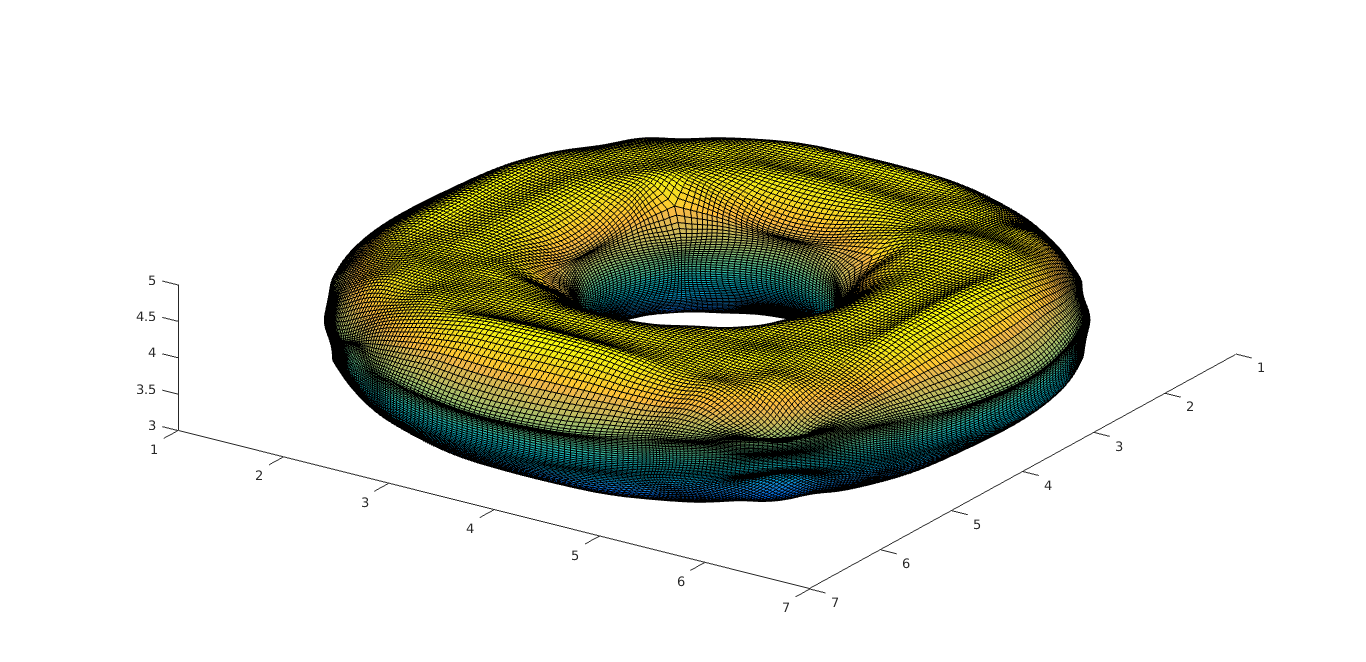
\includegraphics[width = \textwidth]{Pictures/NURBS/torus_from_DC.png}
\caption{A sample result from the Peters' scheme least-squares minimisation surface fitting, using the data provided by the \acs{DC} algorithm for an implicit function describing a torus. The grid lines on the figure are following the constant lines of each parameter value. As they follow the patch edges, corners where other than 4 coarse quads are meeting can be recognized, as for example on the middle of the far side of the torus, on the side that's facing the viewer.}
\label{fig:fittingStructures}
\end{figure}
\todourgent[inline,author=Benni]{@Erik: From Bezier patches to NURBS using degree elevation. Add this to theory and implementation or only here?}

